\documentclass[12pt,letterpaper]{article}
\usepackage{graphicx}
\usepackage{pstricks}
\usepackage[english]{babel}
%\usepackage{pstricks-add}
%\usepackage{pst2pdf}
\usepackage{float}
\graphicspath{{./Figures/}}


\begin{document}
\section{In Read\_data.py}
We begin by reading \texttt{travel\_times\_2011.csv} using csv.DictReader. 
Using \\\textsl{read\_data\_csv}, we then save the trips and travel times data in sparse coordinate matrix form, i.e. (hour (in EDT), link, trips, traveltimes), as \texttt{data\_coo\_form.txt}. 
Next, using \textsl{write\_data\_array},  we write these values to \texttt{data\_trips.csv} and \texttt{data\_travel\_times.csv}. 
For an unknown reason, \textsl{write\_data\_array} introduced a line break in the first hour of the first day of data.
After correcting this break, we reverse the order of the data from the previous step since the data is given in descending order, but we need to write it in ascending order.
Also, to aid in finding submatrices generated by a set of link ids, we transpose \texttt{data\_trips.csv} using \textsl{write\_data\_array\_transpose} to create \texttt{data\_trips\_transpose.csv}.
This is fairly memory intensive due to the scale of the data so we utilized the campus cluster for efficiency. 


Next, we want to pull out the data corresponding to links with at most 30 days worth of data missing; this is done with \textsl{find\_full\_links}. 
We also ran this on the campus cluster.
The list of full link ids is saved under \texttt{full\_link\_ids.txt}.
Similarly, we found all of the links with at most 30 days worth of data; this is done with \textsl{find\_empty\_links} and produces \texttt{empty\_link\_ids.csv}.
We then pull the corresponding data for the full links using write\_full\_link\_data and save into \texttt{full\_link\_trips.json} and \texttt{full\_link\_traveltimes.json}.
Henceforth, \textsl{read\_full\_link\_json} should be used to return the full link ids and their data.

Then, we want to find the periodicity of the full link data. 
By running autocorrelation, we see that the period is 7 days. 
We check the refinement of this by running autocorrelation\_hourly, and verify the 7-day period.
We also checked the periodicity of the travel times and it matches the 7-day period (graph omitted but is saved in Figures\textbackslash).

\begin{figure}[H]
\centering
\includegraphics[width=.9\textwidth]{Autocorrelation_Full_Links.ps}
\end{figure}

\begin{figure}[H]
\centering
\includegraphics[width=.9\textwidth]{Autocorrelation_Full_Links_hourly.ps}
\end{figure}

\section{In Phase1.py}
% Beware NaN is a float so int(NaN) returns error
We group the functions for running Sparse Non-negative Matrix Factorization under \textsl{find\_signatures}.
Then, we save the matrix factorization as \texttt{W\_trips.txt}

Using the old way for calculating error (we include positions corresponding to nan data positions) and running SNMF(traveltimes, rank=50, $\beta=0.1$, $\eta=0.1$, threshold=$0.01$) gave relative error 39.890\%, and for SNMF(trips, rank=50, $\beta=0.1$, $\eta=0.1$, threshold=$0.01$) the error was 28.666\%. 

In the new way, we don't count the guess positions against us and obtain 39.194\% for SNMF(traveltimes, rank=50, $\beta=0.1$, $\eta=0.1$, threshold=$0.01$) and 27.378\% for SNMF(trips, rank=50, $\beta=0.1$, $\eta=0.1$, threshold=$0.01$). 

{\Huge Using the campus cluster, we need to run SNMF with $\beta$, $\eta$, and rank values to determine optimal combination. For now, we continue with rank=50}

After running \textsl{find\_signatures} to produce 
\end{document}